\documentclass{article}

\usepackage{graphicx}
\usepackage{subfig}
\usepackage{amsmath}
\usepackage{listings}
%\usepackage{amsmath,rotating}

\title{One-dimensional Transient Advection/Diffusion Passive Scalar: 15 Point Homework Assignment}

\date{}

\begin{document}

\maketitle

\section{Introduction}
This case provides an implicit simulation study for a one-dimensional time advancement
of a passive scalar (constant properties and advecting velocity) whose partial differential
equation (PDE) includes the effects of time, advection and diffusion (see Section~\ref{s:theory}).

\section{Domain and Initial Condition}
Let the one-dimensional geometry be unity in length with a left inlet value for the passive scalar, $\phi_L = 0$, that corresponds to a Dirichlet condition, while the right domain is a weak, flux-based open boundary. For the right domain, a zero normal gradient for the diffusive flux, $\frac{\partial \phi}{\partial x_j} n_j = 0$, is applied along with advection of this scalar simply leaving the domain . 

For this configuration, let the initial condition be defined as follows,
\begin{align}
\phi(x,t=0) = H e^{\left[{-0.5\left(x-C\right)^2/ \sigma^2}\right]},
\end{align}
where $H$ is the height (1.0), $C$ is the center of the Gaussian profile (1/2), and $\sigma$ is 0.05. Fig.~\ref{fig:IC} represents a sample result at three times (initial time of zero, 0.2, and 0.4). Note that the passive scalar simply advects to the right, and is dissipated via the effects of diffusion.

\begin{figure}[h]
    \centering
    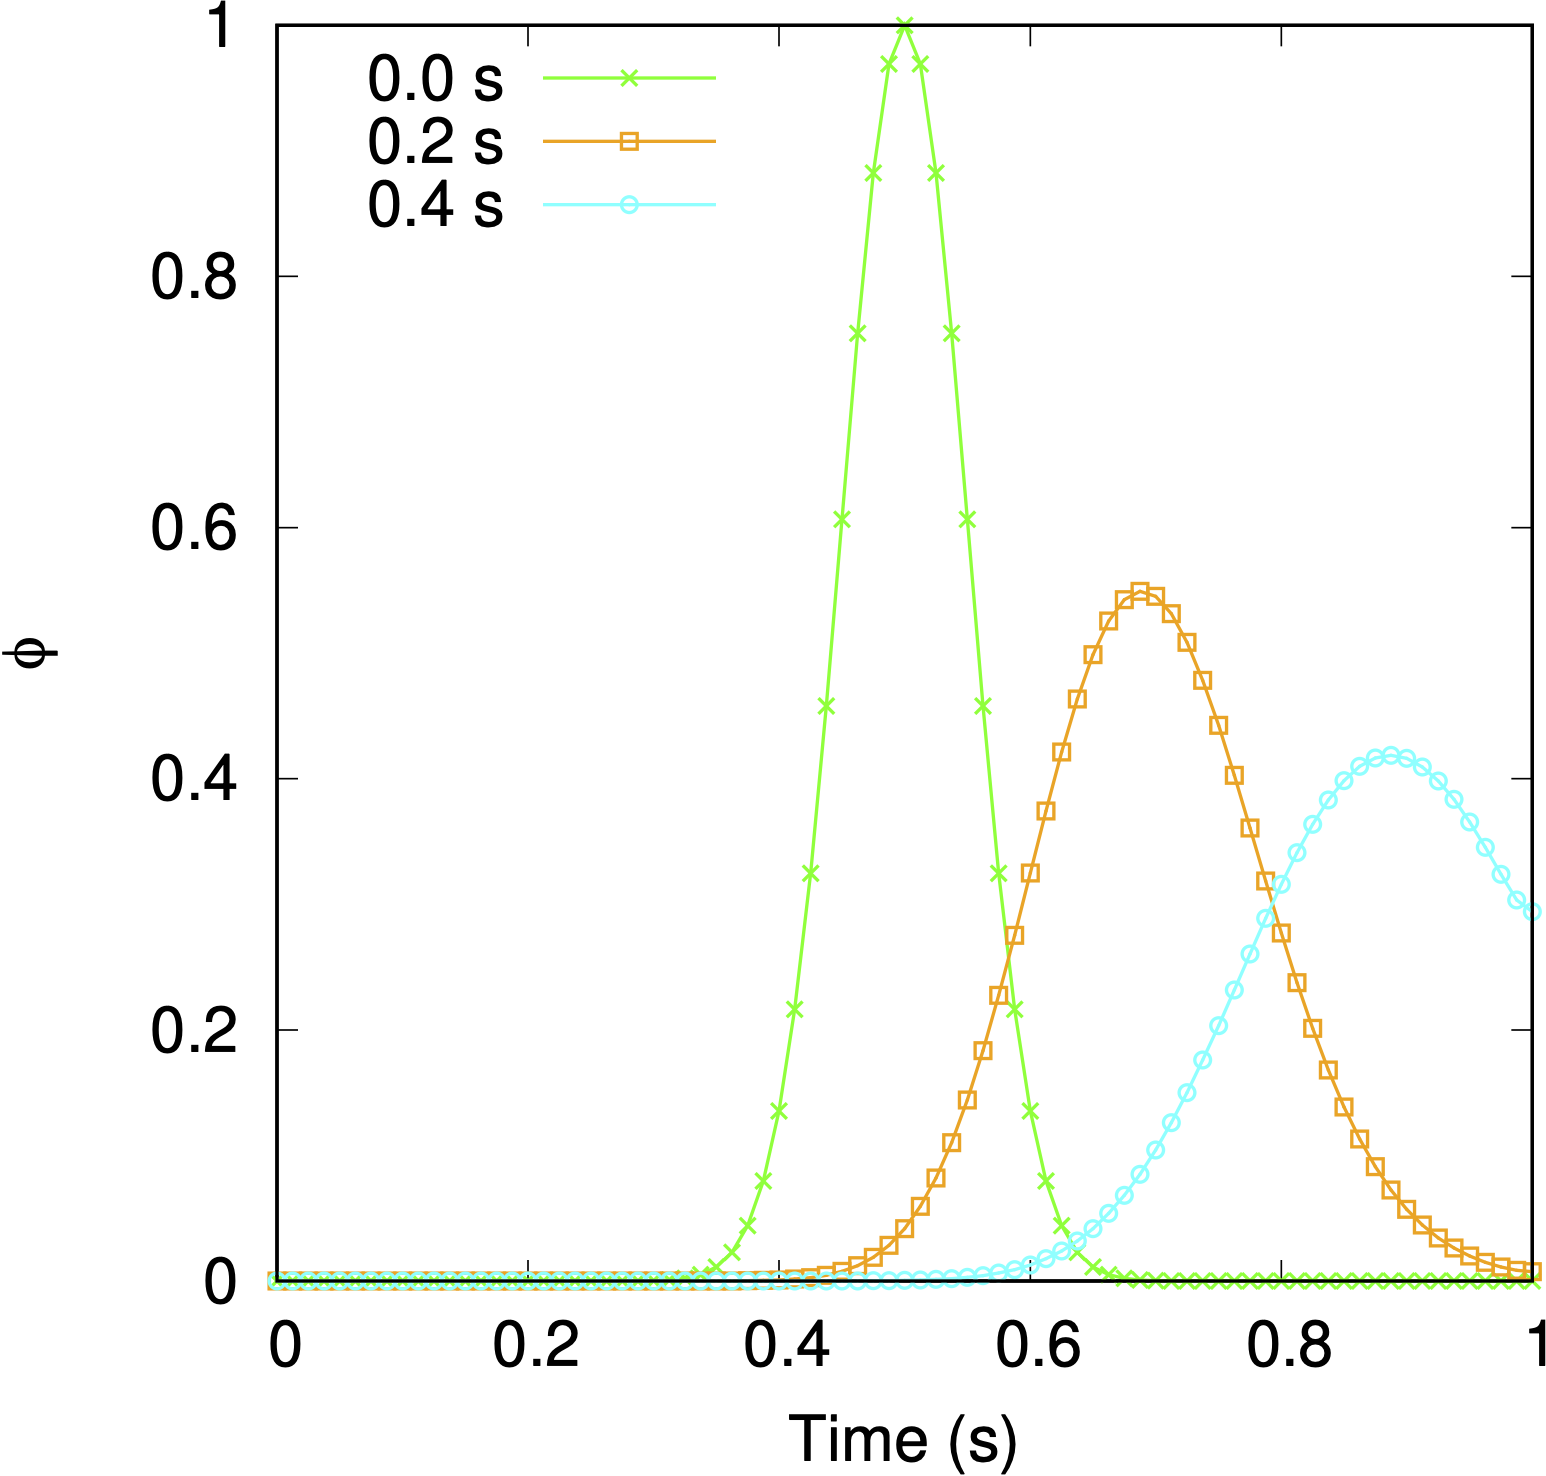
\includegraphics[width=0.5\textwidth]{passiveAdvDiff.png}
    \caption{Gaussian passive scalar at three time planes.}
    \label{fig:IC}
\end{figure}

\section{Theory}
\label{s:theory}
The time varying transport of scalar $\phi$, including with the effects of advection and diffusion, can be represented by the following partial differential equation:

\begin{align}
 \frac {\partial \rho \phi }{\partial t} + \frac{ \partial \rho u_j \phi }{\partial x_j} + \frac{\partial q_j}{\partial x_j} = 0,
\label{eq:contEq}
\end{align} 
where $q_j$ is the diffusive flux vector given by,

\begin{align}
  q_j = -\frac{\mu}{Sc} \frac{\partial \phi}{\partial x_j}.
\label{eq:momEq}
\end{align}

Above, let the Schmidt number, Sc, be unity, with the diffusive flux coefficient, $\frac{\mu}{Sc}$, specified as 0.01.
For this exercise, we will also prescribe a constant density of unity and will solve for the primitive, $\phi$. Finally, the velocity
will also be specified as unity in the positive (left to right) direction.

\subsection{Simulation Specifications}

The above set of equations can be discretized over a one-dimensional coordinate system using a finite difference, finite
volume or finite element method. The supplemental \textit{c++} file provided, fluids\_matrix\_solver\_partial.C, represents
an edge-based, fully implicit implementation for this model equation. While the central advection operator and diffusion operator
have been implemented, an implicit time and upwind advection operator are to be implemented by the student.

Please note that you need not use this sample program if you feel more comfortable with another package such as MATLAB, Maple, etc. Moreover, as we learned in class, a fully explicit scheme may be used -- where time advancement stability may be affected. This is the students choice on methodology used, however, the write-up follows an approach where the supplemental program is to been modified. You will receive points for each question. Note that for the implicit scheme presented, a tri-diagional system is generated that can be solved using a tri-diagonal solver (see below
listing for a sample implementation).  The \textit{c++} file provided can be compiled simply by:

\begin{enumerate}

\item \textit{g++ fluids\_matrix\_solver\_partial.C} -- provides an executable a.out
\item \textit{./a.out} -- will execute the time advancement from zero to 1 second and provide a set of scalar concentrations as a function of space.

\end{enumerate}

You will see that if you compile and run this program, the simulation will throw an exception - requiring that you first implement
an implicit time term contribution. Once you have implemented the time term contribution (using a first-order Backward Euler time integrator described below and in our lectures) you will be able to run the simulation using a central advection operator and plot the simulation results at varying time intervals up to 1 second. After you have implemented the upwind operator, you will also run this configuration, allowing for comparison between the methods. 

\subsection{Solution Procedure}
A simple node-based solution procedure/algorithm for the discretized scheme,

\begin{align}
  \int \rho \frac{\partial \phi}{\partial t} dV + \int \rho u_j \phi n_j dS - \int \frac{\mu}{Sc} \frac{\partial \phi}{\partial x_j} = 0.0,
  \label{eq:phi}
\end{align}
%
can be represented as follows:

\begin{enumerate}

\item Define the one-dimensional set of nodes (or points) that, for this case, may be assumed of constant mesh spacing. 
  
\item Assemble and solve a matrix system for Eq.~\ref{eq:phi} whose velocity, and density
  are set to unity. The effective diffusive flux coefficient is 0.01. The left inflow boundary for $\phi$ is zero and the right boundary is zero flux for diffusion, and simply
  advection out for the scalar. In the sample program, these have been implemented for you.

\item Since the simulation is transient, you will march at a fixed time step. The sample program is set to use a time step
  of 0.1 s, with a total number of points of 21. 
  
  \item Recall that this system is linear, implying that no non-linear iterations need to be applied. The linear system generated can be solved using an iterative method, or via a direct tri-diagonal approach.

\end{enumerate}

\section{Discussion Points and Assignment}

Each question below is assigned two points. The final five points are for the quality of your write-up where it is expected that you mimic this write-up (see below for more details). 

\begin{itemize}

\item If using the sample program edge-based finite volume procedure provided, add the implicit time term specification
  for a first-order backward Euler scheme.
  For this discretization scheme, the time term is evaluated at the nodes and is simply,
  \begin{align}
    \rho\frac{\phi_j^{n+1} - \phi_j^n}{\Delta t} V_j.
  \end{align}
  Above $j$ is the node number, and $V_j$ is the control volume. Although we have only defined a one-dimensional
  set of nodes, we can view an area as unity (effectively a unity length in the y- and z-directions), thereby
  providing a proper volume for each cell. The implicit term, here assuming matrix $A$, solution vector $\phi$ and right-hand-side, $b$, can be written $Ax=b$ where $A$ includes terms that scale $\phi^{n+1}$. 
  
  If you are using your own program, implement the time, diffusion, and advection contribution.

\item If you used 21 points, i.e., the size exercised in the sample program, along with properties (and velocity) noted above, what is the maximum Courant number over all nodes for the 0.01 s configuration? Recall that the Courant number is defined as: $\frac{u \Delta t}{\Delta x}$. Comment on the stability of your method using this time step. Again, using roughly 21 points, along with properties (and velocity) noted above, what is the maximum Peclet number (the Peclet number is defined as: $\frac{\rho u \Delta x}{\mu/Sc}$).

\item Run a simulation with the roughly 21 point specification (using the central, i.e., Galerkin advection operator) and plot the
  scalar value starting at 0.0 seconds, while terminating at 1.0 seconds using 0.1 s time intervals. Comment on dispersion or
  dissipation errors that you might see. This plot should resemble what is shown in Fig.~\ref{fig:IC}.
  
\item Implement a first-order upwind scheme (in the provided code base, const bool upwind = true; ) and replicate the
  above experiment - again creating a new set of temporal plots. What do you see that is different?

\item Finally, change any property (density or diffusive flux coefficient), velocity magnitude, number of points --
  or even the direction of velocity and provide a transient set of plots as performed above. Comment on what you
  see by this change. Note that if you do change the flow direction, the left and right boundary conditions are swapped. If you implemented the upwind method properly, no other changes should be required.

\end{itemize}

As noted, there are many tools that can be used to solve this problem ranging from your own program with a linear
solve (see below for a tri-diagonal solver details), the program that was provided, a scientific programing platform
such as MATLAB, or even a spread sheet application!

\newpage

\begin{lstlisting}[caption={This is a tri-diagonal implicit matrix solve routine (also
known as the Thomas Algorithm) and is suitable for solving a diagonal dominant matrix system. For structured
three-dimensional applications, alternating sweep directions can be combined with the tri-diagonal solve. In this 
implementation, the matrix coefficients are modified and are not intended to be re-used for each subsequent 
iteration.},captionpos=b]

void tdma(int mSize, NaluOneDMatrixSystem *ns, double *u) {
  
  // forward
  for ( int k = 1; k < mSize; ++k ) {
    const double m = ns[k].Aw_/ns[k-1].Ap_;
    ns[k].Ap_ -= m*ns[k-1].Ae_;
    ns[k].rhs_ -= m*ns[k-1].rhs_;
  }

  // backward
  u[mSize-1] = ns[mSize-1].rhs_/ns[mSize-1].Ap_;
  for ( int k = mSize-2; k >= 0; --k ) {
    u[k] = (ns[k].rhs_ - ns[k].Ae_*u[k+1])/ns[k].Ap_;
  }
}

\end{lstlisting}

\section{Specified Code Implementation Notes}
In the code base provided, you will see that a set of nodes and edges have been created. Data from velocity, $\phi$, coordinates, and properties reside at the nodes. Surface-based contributions are assembled via an iteration over edges with an assumed area vector orientation of left to right. For each integration point within the edge, a "left" and "right" connectivity has been defined. The left and right node for each edge is accessed by the "lrscv" data structures. The coordinates and the left and right node for each edge can be extracted by "coords[il] and coords[ir]", respectively. Nodal loops can extract nodal data directly for node k. 

A one-dimensional matrix structure has been created where each row has a left, central, and right coefficient, $A_w$, $A_p$, and $A_e$, in addition to a right-hand side vector, $rhs$. It's interesting to consider that the time, advection and diffusion kernels for this sample code base would be exactly the same for an unstructured capability, noting that only the matrix connectivity mapping and scatter operation would need to be changed (in addition to the edge data structure being created). 

Remember that you can easily derive this matrix system on paper; if you are confused by the matrix assembly abstractions presented, simply "hand code" the contributions and solve the system for each time step.

\section{Required Report Attributes}
Please create a short write-up (roughly five pages) that may be completed with up to three students in each group. Please address all of the questions addressed above. Your report should include a brief overview of the equation solved, and the numerical
techniques used along with answering each of the questions posed above. Your report should also include the two plots at
the coarse 21-point simulation (central and upwind), in addition to a plot for the parameter you varied. Finally, provide your sample program that you used for your study. 

\section{Life Vest Options}
Should you be completely confused by either a code implementation or "hand code" approach, you may reach out for a fully implemented code base where you can conduct the above requirements. However, a three point penalty will be assessed where the maximum grade achievable would be 12 points.

\end{document}
